% !TeX spellcheck = pt_BR

%%%%%%%%%%%%%%%%%%%%%%%%%%%%%%%%%%%%%%%%%%%%%%%
% Modelo adaptado do template original de
% Ted Pavlic (http://www.tedpavlic.com)
% Todos os créditos a ele.
%
% Na versão atual, o que foi modificado
% do original:
% Ajusta a numeração das questões e
% passa para português.
% Além de separar as configurações
% em um arquivo .cls separado.
%
% Crédito ao Roberto por ter feito
% a maior parte do trabalho de passar
% para o português e fazer outros
% ajustes para a versão atual deste template.
%%%%%%%%%%%%%%%%%%%%%%%%%%%%%%%%%%%%%%%%%%%%%%%


%----------------------------------------------------------------------------------------
%	PACKAGES E OUTRAS CONFIGURAÇÕES
%----------------------------------------------------------------------------------------

\documentclass{homeworkclass}

\usepackage{animate}


\usepackage{myMacros}


\hmwkTitle{Lista\ de\ Exercícios \#4}
\hmwkDueDate{Segunda,\ 05\ de\ Julho,\ 2019}
\hmwkClass{Elementos de Processamento de 	Sinais}
\hmwkClassTime{Segundas e Quartas (e Sextas): 08:00--10:00}
\hmwkClassInstructor{Prof.\ Sergio Lima Netto}
\hmwkAuthorName{Vinicius Mesquita de Pinho}
\hmwkAuthorShortName{Vinicius Mesquita}

\begin{document}

\maketitle

%----------------------------------------------------------------------------------------
%	SUMÁRIO
%----------------------------------------------------------------------------------------

%\setcounter{tocdepth}{1} % Uncomment this line if you don't want subsections listed in the ToC

\clearpage
\newpage
%\tableofcontents
%\newpage

%----------------------------------------------------------------------------------------
%	QUESTÃO 1
%----------------------------------------------------------------------------------------

% To have just one problem per page, simply put a \clearpage after each problem



\begin{homeworkProblem}
	Projeto de um filtro rejeite-faixas digital através da aproximação de Chebyshev. \\
	
	O projeto será da seguinte maneira:
	\begin{itemize}
		\item Conversão das frequências de operação para as frequências digitais (entre $0$ e $2\pi$).
		\item Realização do \textit{prewarp} das frequências, ou seja, $\Omega_{a} = (2/T)\tan(w/2)$, obtendo as frequências analógicas correspondentes.
		\item Verificação se o filtro analógico resultante é geometricamente simétrico. Caso não seja, fazer a adequação.
		\item Normalização do filtro, para calculo de $H(s^{\prime})$, o seu equivalente passa-baixas analógico.
		\item Desnormalização do filtro passa-baixas calculado para o tipo de filtro desejado, neste caso rejeita-faixa, calculo do $H(s)$.
		\item Transformação do filtro analógico calculado para o domínio digital atráves da transformação bilinear, calculando $H(z)$.
	\end{itemize}
	
	\paragraph{A aproximação de Chebyshev:} Esse método apresenta melhor aproveitamento das especificações em banda passante, pois sua função de atenuação é:
	\begin{equation}
	|A(\jrm \Omega^{\prime})|^{2} = 1 + \epsilon^{2}C_{n}^{2}\left(\Omega^{\prime}\right),
	\end{equation}
	onde 
	\begin{equation}
	C_n(\Omega')=
	\begin{cases}
	\textrm{cos}[n\textrm{cos}^{-1}(\Omega')], \quad & 0 \leq \Omega' \leq 1\\
	\textrm{cosh}[n\textrm{cosh}^{-1}(\Omega')], & \Omega'>1.
	\end{cases}
	\label{eq:2}
	\end{equation}
	A equação~\eqref{eq:2} mostra que a função de Chebyshev $C_{n}$ tem característica oscilatória para $0 \leq \Omega^{\prime} \leq 1$, assim fazendo melhor aproveitamento das especificações na banda passante do filtro.
	
	\paragraph{As especificações do filtro desejado:} $A_{p1} = 1$~dB, $A_{p2} = 2$~dB, $A_{r} = 40$~dB, $\Omega_{p1} = 850$~Hz, $\Omega_{r1} = 980$~Hz, $\Omega_{p2} = 1020$~Hz, $\Omega_{r2} = 1150$~Hz, $\Omega_{s} = 10$~kHz.
	
	Escolhi um exemplo em que as especificações possuem atenuções diferentes nas bandas passantes.
	
	\pagebreak
	A Figura~\ref{fig:fig1} mostra a magnitude da resposta em frequência do filtro analógico passa-baixas normalizado, calculado pela aproximação de Chebyshev. Com os coeficientes deste filtro, foi realizado sua desnormalização, gerando um filtro rejeita-faixa da Figura~\ref{fig:fig2}. Porém, esses filtros projetados ainda são analógicos. Através da transformação bilinear 
	\begin{equation*}
	s = \frac{2(z-1)}{T(z+1)},
	\end{equation*}
	temos o filtro digital rejeita-faixa da Figura~\ref{fig:fig3}.
	
	

\begin{figure}[!h]
	\centering
	\subfloat[Filtro passa-baixas analógico.]{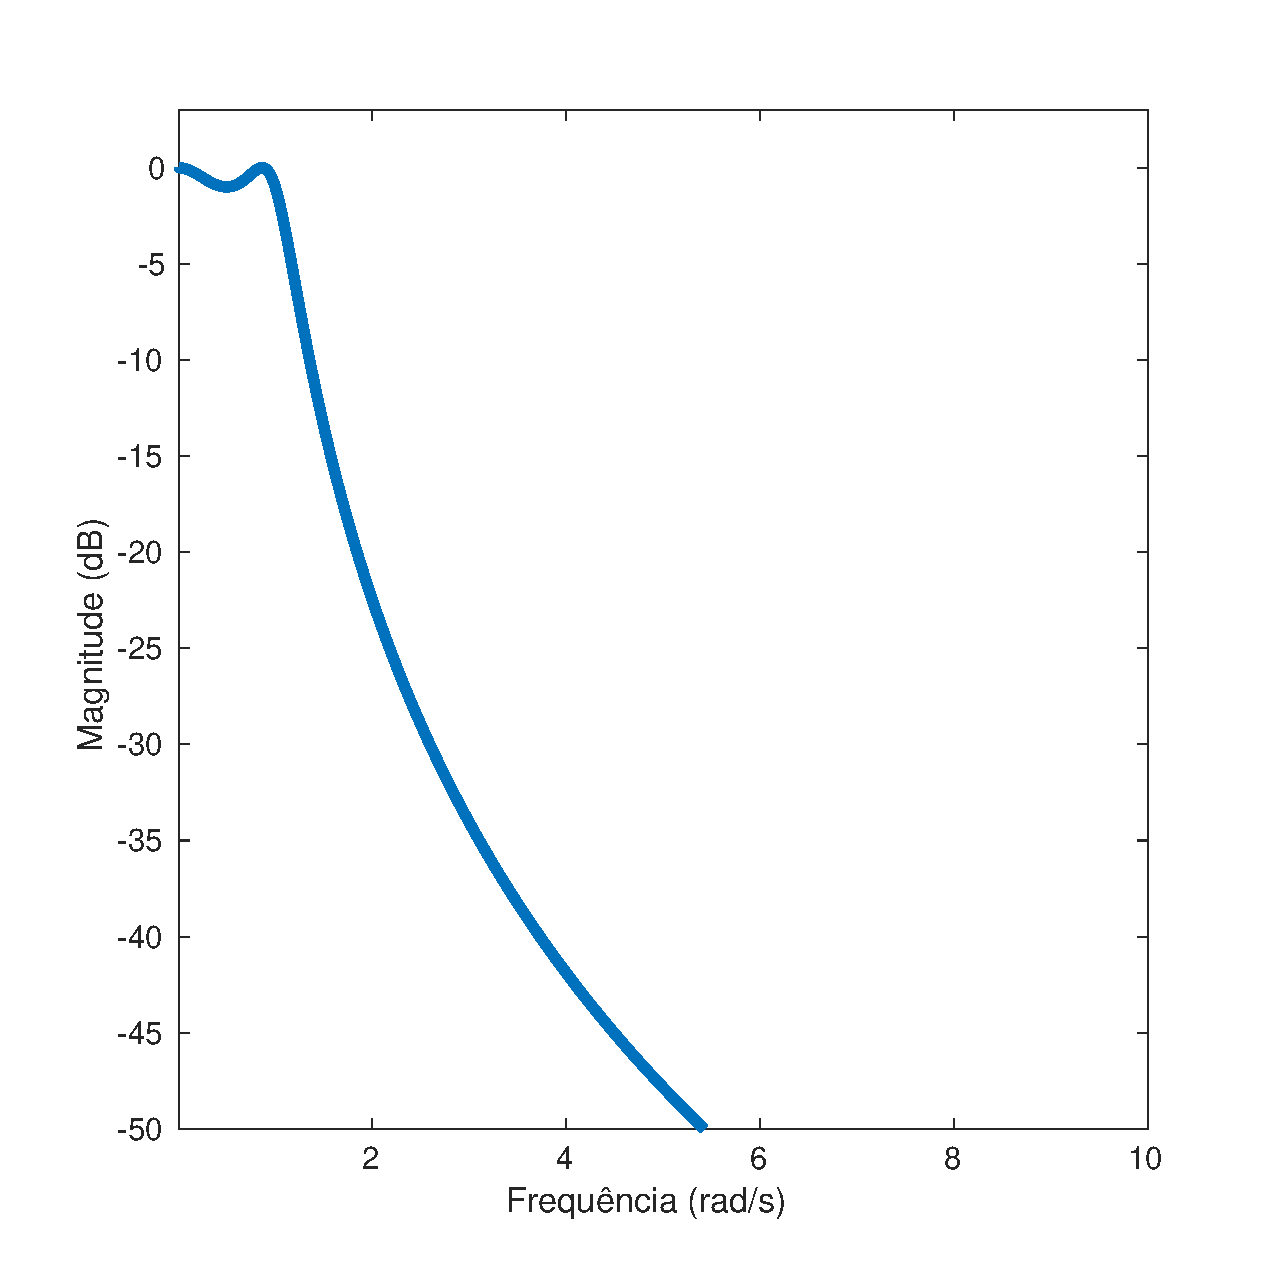
\includegraphics[width=0.46\linewidth]{figs/fig1}\label{fig:fig1}}
	~
	\subfloat[Filtro rejeita-faixa analógico.]{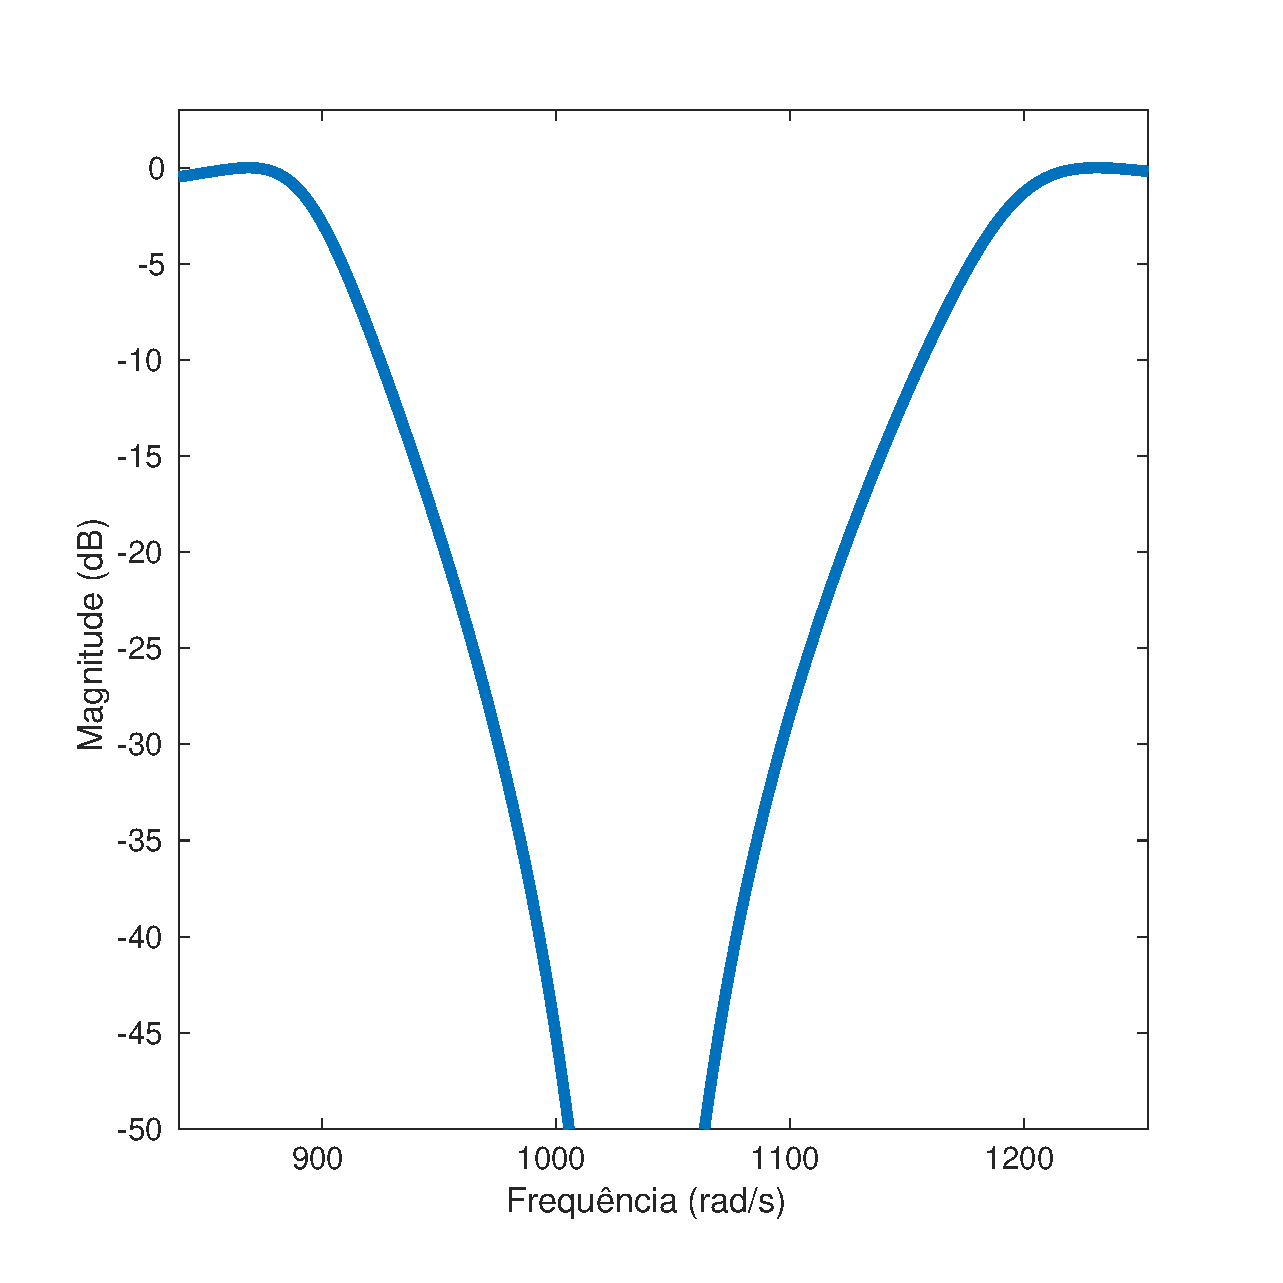
\includegraphics[width=0.46\linewidth]{figs/fig2}	\label{fig:fig2}}
	\\
	\subfloat[Filtro passa-baixas digital.]{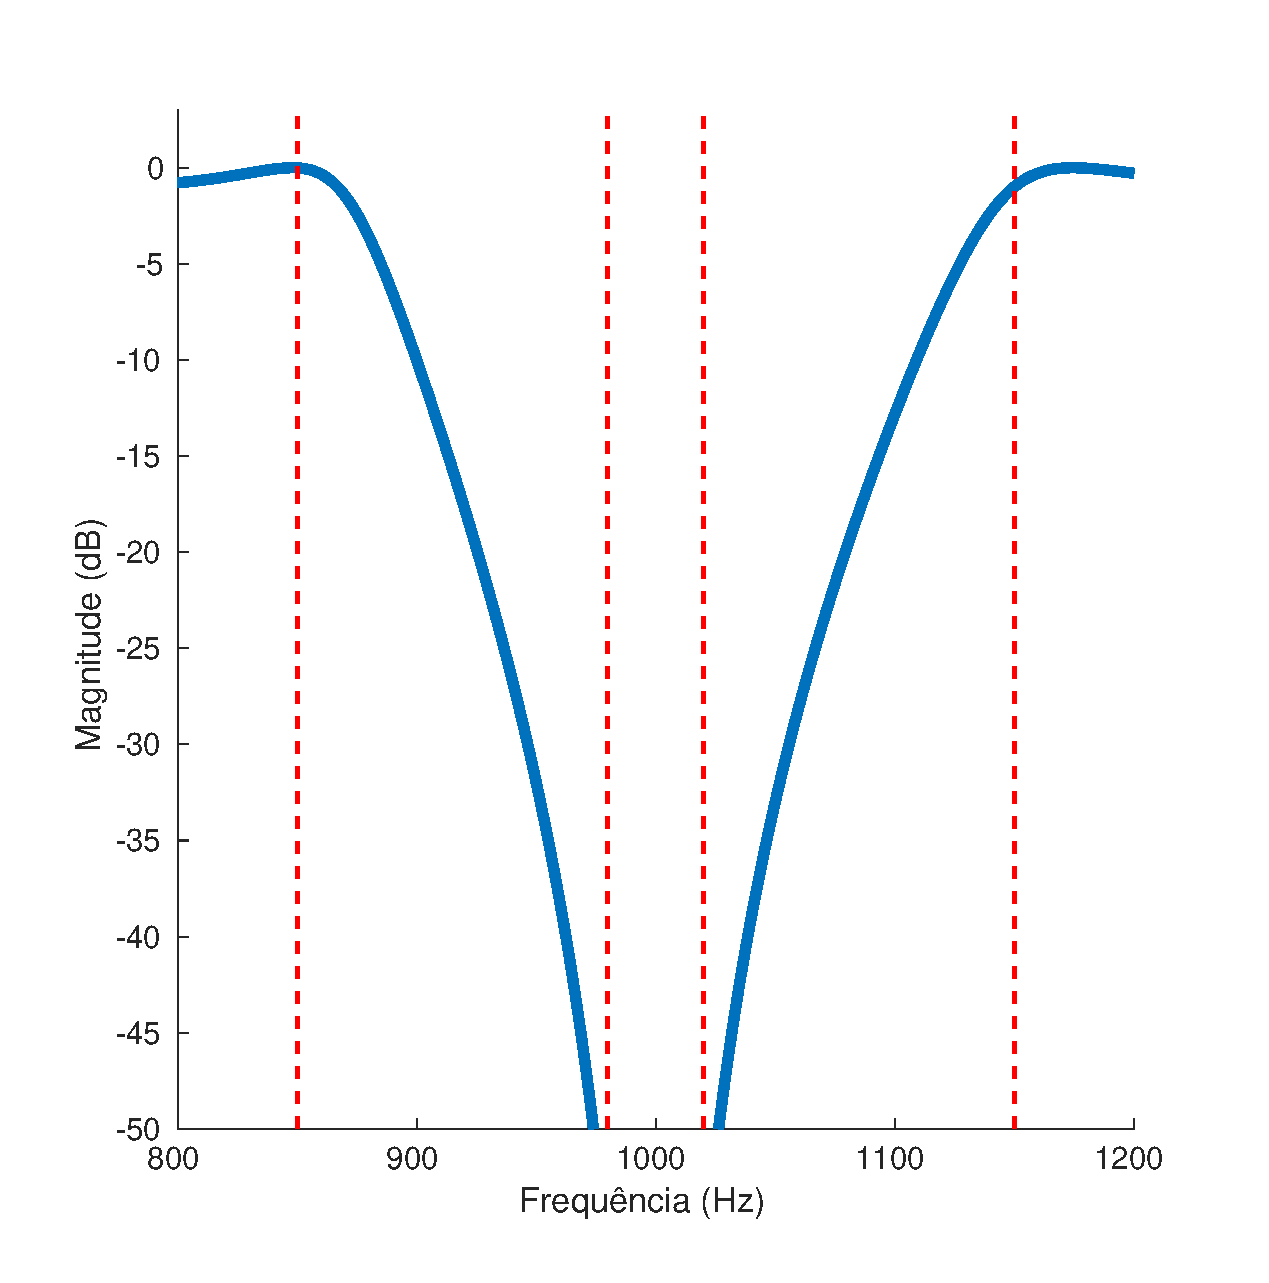
\includegraphics[width=0.46\linewidth]{figs/fig3}	\label{fig:fig3}}
	
	\caption{Etapas para design do filtro digital rejeita-faixa.}
	\label{fig:total}
\end{figure}
	



\end{homeworkProblem}

\end{document}